%%%%%%%%%%%%%%%%%%%%%%%%%%%%%%%%%%%%%%%%%%%%%%%%%%%%%%%%
%                IAML 2020 Assignment 1                %
%                                                      %
%                                                      %
% Authors: Oisin Mac Aodha and Octave Mariotti         %
% Using template from: Michael P. J. Camilleri and     %
% Traiko Dinev.                                        %
%                                                      %
% Based on the Cleese Assignment Template for Students %
% from http://www.LaTeXTemplates.com.                  %
%                                                      %
% Original Author: Vel (vel@LaTeXTemplates.com)        %
%                                                      %
% License:                                             %
% CC BY-NC-SA 3.0                                      %
% (http://creativecommons.org/licenses/by-nc-sa/3.0/)  %
%                                                      %
%%%%%%%%%%%%%%%%%%%%%%%%%%%%%%%%%%%%%%%%%%%%%%%%%%%%%%%%

%--------------------------------------------------------
%   IMPORTANT: Do not touch anything in this part
\documentclass[12pt]{article}
%%%%%%%%%%%%%%%%%%%%%%%%%%%%%%%%%%%%%%%%%
% Cleese Assignment
% Structure Specification File
% Version 1.0 (27/5/2018)
%
% This template originates from:
% http://www.LaTeXTemplates.com
%
% Author:
% Vel (vel@LaTeXTemplates.com)
%
% License:
% CC BY-NC-SA 3.0 (http://creativecommons.org/licenses/by-nc-sa/3.0/)
% 
%%%%%%%%%%%%%%%%%%%%%%%%%%%%%%%%%%%%%%%%%

%----------------------------------------------------------------------------------------
%	PACKAGES AND OTHER DOCUMENT CONFIGURATIONS
%----------------------------------------------------------------------------------------

\usepackage{lastpage} % Required to determine the last page number for the footer
\usepackage{graphicx} % Required to insert images
\setlength\parindent{0pt} % Removes all indentation from paragraphs
\usepackage[most]{tcolorbox} % Required for boxes that split across pages
\usepackage{booktabs} % Required for better horizontal rules in tables
\usepackage{listings} % Required for insertion of code
\usepackage{etoolbox} % Required for if statements
\usepackage{geometry} % Required for adjusting page dimensions and margins
\usepackage[utf8]{inputenc} % Required for inputting international characters
\usepackage[T1]{fontenc} % Output font encoding for international characters
\usepackage{fancyhdr} % Required for customising headers and footers
\usepackage{xspace}
\usepackage{booktabs}
\usepackage[colorlinks]{hyperref}
\usepackage{etoolbox}

\newcommand{\ie}{i.e.\@\xspace}
\newcommand{\eg}{e.g.\@\xspace}
\newcommand{\notemark}[1]{\textcolor{blue}{N.B.\ \emph{#1}}}
\newcommand{\noteself}[1]{\textcolor{red}{Thought: \emph{#1}}}
\newcommand{\note}[1]{\emph{\textbf{N.B.}\@\xspace#1}}
\newcommand{\hint}[1]{\emph{Hint: #1}}
\newcommand{\half}{$\frac{1}{2}$ }

\newbool{clearnext}		%Running Counter to see if clearing the page or not in the next subquestion.
\newbool{clearon}		%Parameter for specifying whether we will be clearing or not.
\newbool{authoron}		%Parameter to specify whether to show author or not

%----------------------------------------------------------------------------------------
%	Standard Template
%----------------------------------------------------------------------------------------
\geometry{
	paper=a4paper, % Change to letterpaper for US letter
	top=3cm, % Top margin
	bottom=3cm, % Bottom margin
	left=2.5cm, % Left margin
	right=2.5cm, % Right margin
	headheight=14pt, % Header height
	footskip=1.4cm, % Space from the bottom margin to the baseline of the footer
	headsep=1.2cm, % Space from the top margin to the baseline of the header
	%showframe, % Uncomment to show how the type block is set on the page
}
\pagestyle{fancy} % Enable custom headers and footers

%----------------------------------------------------------------------------------------
%	My Changes
%----------------------------------------------------------------------------------------
\lhead{\small\assignmentClass}
\chead{}
\ifbool{authoron}{\rhead{\small{\assignmentAuthorName}}}{\rhead{}}

\lfoot{} % Left footer
\cfoot{} % Centre footer
\rfoot{\small Page\ \thepage\ of\ \pageref*{LastPage}} % Right footer

\renewcommand\headrulewidth{0.5pt} % Thickness of the header rule

%----------------------------------------------------------------------------------------
%	MODIFY SECTION STYLES
%----------------------------------------------------------------------------------------

\usepackage{titlesec} % Required for modifying sections

%------------------------------------------------
% Section

\titleformat
{\section} % Section type being modified
[block] % Shape type, can be: hang, block, display, runin, leftmargin, rightmargin, drop, wrap, frame
{\Large\bfseries} % Format of the whole section
{\assignmentQuestionName~\thesection} % Format of the section label
{6pt} % Space between the title and label
{} % Code before the label

\titlespacing{\section}{0pt}{0.5\baselineskip}{0.5\baselineskip} % Spacing around section titles, the order is: left, before and after

%------------------------------------------------
% Subsection

\titleformat
{\subsection} % Section type being modified
[block] % Shape type, can be: hang, block, display, runin, leftmargin, rightmargin, drop, wrap, frame
{} % Format of the whole section
{\bf{\arabic{section}.\arabic{subsection}}} % Format of the section label
{4pt} % Space between the title and label
{} % Code before the label

\titlespacing{\subsection}{0pt}{0.5\baselineskip}{0.5\baselineskip} % Spacing around section titles, the order is: left, before and after

% \renewcommand\thesubsection{(\alph{subsection})}
\renewcommand\thesubsection{\arabic{section}.\arabic{subsection}}

%----------------------------------------------------------------------------------------
%	CUSTOM QUESTION COMMANDS/ENVIRONMENTS
%----------------------------------------------------------------------------------------

% Environment to be used for each question in the assignment
\newenvironment{question}[1]{
	\ifbool{clearon}{\clearpage}{}
	\global\setbool{clearnext}{false}
	\vspace{0.5\baselineskip} % Whitespace before the question
	\section{: #1}
	\lfoot{\small\itshape\assignmentQuestionName~\thesection~continued on next page\ldots} % Set the left footer to state the question continues on the next page, this is reset to nothing if it doesn't (below)
}{
	\lfoot{} % Reset the left footer to nothing if the current question does not continue on the next page
}

%------------------------------------------------

% Environment for inter-subquestion texts (no arguments)
\newenvironment{interquestiontext}{
	\ifbool{clearon}{\ifbool{clearnext}{\clearpage}{}}{}
	\global\setbool{clearnext}{false}
}{
}

%------------------------------------------------


%------------------------------------------------

% Environment for subquestions, takes 1 argument - the name of the section
\newenvironment{subquestion}[1]{
	\ifbool{clearon}{\ifbool{clearnext}{\clearpage}{}}{}
	\global\setbool{clearnext}{true}
	\subsection{#1}
}{
}

%------------------------------------------------

% Command to print a question sentence
\newcommand{\questiontext}[1]{
	\textbf{#1}
	\vspace{0.5\baselineskip} % Whitespace afterwards
	\global\setbool{clearnext}{false}
}

%------------------------------------------------
% Command to print a  Marking Scheme box.
\newcommand{\marking}[1]{
	\begin{tcolorbox}[colback=green!5!white,enhanced]
		\textbf{Marking Scheme:}#1
	\end{tcolorbox}
}

%------------------------------------------------

% Command to print a box that breaks across pages with the space for a student to answer
\newenvironment{model}[1]{
\begin{tcolorbox}[enhanced]
\textbf{Model Answer}:
#1
}
{
\end{tcolorbox}
}

\newenvironment{answerbox}[1]{
\begin{tcolorbox}[enhanced, height=#1]
}
{
\end{tcolorbox}
}



%------------------------------------------------

% Command to print an assignment section title to split an assignment into major parts
\newcommand{\assignmentSection}[1]{
	{
		\centering % Centre the section title
		\vspace{2\baselineskip} % Whitespace before the entire section title
		
		\rule{0.8\textwidth}{0.5pt} % Horizontal rule
		
		\vspace{0.75\baselineskip} % Whitespace before the section title
		{\LARGE \MakeUppercase{#1}} % Section title, forced to be uppercase
		
		\rule{0.8\textwidth}{0.5pt} % Horizontal rule
		
		\vspace{\baselineskip} % Whitespace after the entire section title
	}
}

%----------------------------------------------------------------------------------------
%	TITLE PAGE
%----------------------------------------------------------------------------------------

\title{
	\thispagestyle{empty} 		% Suppress headers and footers
	\vspace{0.01\textheight} 	% Whitespace before the title
        \hfill {\normalsize \it Ver.~1.0.0}\\
	\textbf{\assignmentClass:\\ \assignmentTitle}\\[4pt]
	\ifbool{authoron}{\assignmentAuthorName}{
	\ifdef{\assignmentDueDate}{{\small Due\ on\ \assignmentDueDate}\\}{}
	{\large \textit{\assignmentWarning}}
	\vspace{0.01\textheight}} % Whitespace before the author name
}

\ifbool{authoron}{\author{Student: \textbf{\assignmentAuthorName}}}{}
\date{} % Don't use the default title page date field

% by Hiroshi
\usepackage{bm}
\newcommand{\VEC}[1]{\ensuremath{\bm{#1}}}
\newcommand{\refQ}[1]{Question~\ref{#1}}
\hypersetup{linkcolor=blue}




% Options for Formatting Output

\global\setbool{clearon}{true} %
\global\setbool{authoron}{true} %



\newcommand{\assignmentQuestionName}{Question}
\newcommand{\assignmentTitle}{Assignment\ \#1}

\newcommand{\assignmentClass}{IAML -- INFR10069 (LEVEL 10)}

\newcommand{\assignmentWarning}{NO LATE SUBMISSIONS} % 
\newcommand{\assignmentDueDate}{Tues,\ October\ 20,\ 2020 @ 16:00}
%--------------------------------------------------------


%%%%%%%%%%%%%%%%%%%%%%%%%%%%%%%%%%%%%%%%%%%%%%%%%%%%%%%
%
% NOTE: YOU NEED TO ENTER YOUR STUDENT ID BELOW.
%
%%%%%%%%%%%%%%%%%%%%%%%%%%%%%%%%%%%%%%%%%%%%%%%%%%%%%%%%
%--------------------------------------------------------
% IMPORTANT: Specify your Student ID below. You will need to uncomment the line, else compilation will fail. Make sure to specify your student ID correctly, otherwise we may not be able to identify your work and you will be marked as missing.
\newcommand{\HAO ZHOU}{s1862323}
%--------------------------------------------------------



\begin{document}
\maketitle
\thispagestyle{empty}







%%%%%%%%%%%%%%%%%%%%%%%%%%%%%%%%%%%%%%%%%%%%%%%%%%%%%%%%%%%%%%%%%%%%%%%%%%%%%%
%============================================================================%
%%%%%%%%%%%%%%%%%%%%%%%%%%%%%%%%%%%%%%%%%%%%%%%%%%%%%%%%%%%%%%%%%%%%%%%%%%%%%%
\clearpage

\begin{question}{(22 total points) Linear Regression}

\questiontext{In this question we will fit linear regression models to data.}



%
%
\begin{subquestion}{(3 points) Describe the main properties of the data, focusing on the size, data ranges, and data types.   
}


\begin{answerbox}{10em}
size: 50 entries,range index from 0 to 49, 2 columns and 50 rows.
data ranges: revision time is from 2.723 to 48.011, exam_score is from 14.731 to 94.945. index range is from 0 to 49.
data types: float64(2)
memory usage: 880.0 bytes
<class 'pandas.core.frame.DataFrame'>
revision_time    50 non-null float64
exam_score       50 non-null float64
\end{answerbox}



\end{subquestion}




%
%
\begin{subquestion}{(3 points) Fit a linear model to the data so that we can predict \texttt{exam\_score} from \texttt{revision\_time}. 
Report the estimated model parameters $\mathbf{w}$. 
Describe what the parameters represent for this 1D data. 
For this part, you should use the sklearn implementation of \href{https://scikit-learn.org/0.19/modules/generated/sklearn.linear_model.LinearRegression.html}{Linear Regression}.\\
\hint{By default in sklearn \texttt{fit\_intercept = True}. Instead, set \texttt{fit\_intercept = False} and pre-pend $1$ to each value of $x_i$ yourself to create $\boldsymbol{\phi}(x_i) = [1, x_i]$. 
}
}


\begin{answerbox}{10em}
Your Answer Here
The coefficient of linear regression is 1.44114091 and the intercept is 17.89768026.
\end{answerbox}



\end{subquestion}



%
%
\begin{subquestion}{(3 points) Display the fitted linear model and the input data on the same plot.
}


\begin{answerbox}{35em}
This image shows the fitted linear model and the input data on the same plot
\begin{center}
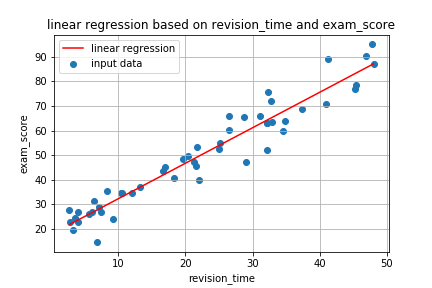
\includegraphics[width = 0.7\textwidth]{Question 1c.jpg}
\end{center}
\end{answerbox}



\end{subquestion}



%
%
\begin{subquestion}{(3 points) Instead of using sklearn, implement the closed-form solution for fitting a linear regression model yourself using numpy array operations.  
Report your code in the answer box.
It should only take a few lines (i.e. <5).\\ 
\hint{Only report the relevant lines for estimating $\mathbf{w}$ e.g. we do not need to see the data loading code. You can write the code in the answer box directly or paste in an image of it. }
}


\begin{answerbox}{20em}
code(start)
X = np.insert(regressionData.loc[:,['revision_time']].values, 0, 1, axis=1)    
X_ = np.linalg.inv(X.T.dot(X))
w = X_.dot(X.T).dot(regressionData.loc[:,['exam_score']].values)
y_pred = X.dot(w)
(finish)
Explanation: equation = (X^t*X)^-1 * X^t * y
X is the revision_time, X.T is the transpose of X, X_ is the inverse of transpose of (X multiply with X), y = exam_score


\end{answerbox}



\end{subquestion}



%
%
\begin{subquestion}{(3 points) Mean Squared Error (MSE) is a common metric used for evaluating the performance of regression models. 
Write out the expression for MSE and list one of its limitations. \\
\hint{For notation, you can use $y$ for the ground truth quantity and $\hat{y}$ (\texttt{\$\textbackslash{}hat\{y\}\$} in latex) in place of the model prediction.}
}


\begin{answerbox}{10em}
Mean squared error expression:$$ 
MSE = {/frac{1}{n}\sum_{i=1}^{n}(y_{i}-\hat{y_{i}})^{2}}
$$
The limitation is related to the distribution of the data. The exceptional points would increase the MSE. MSE is also prone to outliers as it uses the same concept of using mean in computing each error value. The extreme large point or small point will make MSE unreliable.
\end{answerbox}



\end{subquestion}


 
%
%
\begin{subquestion}{(3 points) Our next step will be to evaluate the performance of the fitted models using Mean Squared Error (MSE). 
Report the MSE of the data in \texttt{regression\_part1.csv} for your prediction of \texttt{exam\_score}.
You should report the MSE for the linear model fitted using sklearn and the model resulting from your closed-form solution. 
Comment on any differences in their performance. 
}


\begin{answerbox}{10em}
The MSE of linear model fitted using sklearn:30.98547261454128
The MSE of linear model using numpy function:30.985472614541287
The difference exist in the 14th decimal place,because when we using sklearn calculated w slightly different with w calculated by using numpy fucntion.Using sklearn way w is [17.897680258350174,1.441140905437971] and numpy way w is [17.897680258350192,1.4411409054379702]. It is the reason why the decimal place is different in MSE. Also, because it's numerically unstable in matrix multiplication X^T * X and this make the results extremely unstable and then MSE got difference in 14th decimal place. But because the difference is extremely small we can ignore it.Hence the MSE is the same.
\end{answerbox}



\end{subquestion}




%
%
\begin{subquestion}{(4 points) Assume that the optimal value of $w_0$ is $20$, it is not but let's assume so for now. 
Create a plot where you vary $w_1$ from $-2$ to $+2$ on the horizontal axis, and report the Mean Squared Error on the vertical axis for each setting of $\mathbf{w} = [w_0, w_1]$ across the dataset. 
Describe the resulting plot. Where is its minimum? Is this value to be expected?\\ 
\hint{You can try 100 values of $w_1$ i.e. \texttt{w1 = np.linspace(-2,2, 100)}.}
}


\begin{answerbox}{35em}
The minimum value of w1 is 32.48096161535148 and the index of it is 83
This image shows MSE values based on different w1
\begin{center}
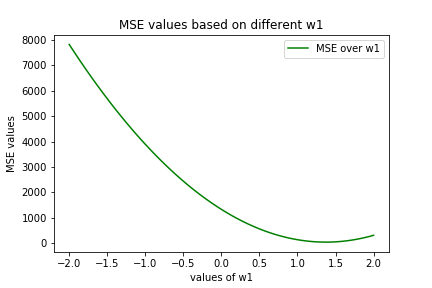
\includegraphics[width = 0.7\textwidth]{Question 1g.jpg}
\end{center}
\end{answerbox}



\end{subquestion}


 
\end{question}





%%%%%%%%%%%%%%%%%%%%%%%%%%%%%%%%%%%%%%%%%%%%%%%%%%%%%%%%%%%%%%%%%%%%%%%%%%%%%%
%============================================================================%
%%%%%%%%%%%%%%%%%%%%%%%%%%%%%%%%%%%%%%%%%%%%%%%%%%%%%%%%%%%%%%%%%%%%%%%%%%%%%%
\clearpage



\begin{question}{(18 total points) Nonlinear Regression}

\questiontext{In this question we will tackle regression using basis functions.}




%
%
\begin{subquestion}{(5 points) Fit four different polynomial regression models to the data  by varying the degree of polynomial features used i.e. $M = 1$ to $4$.
For example, $M=3$ means that $\boldsymbol{\phi}(x_i) = [1, x_i, x_i^2, x_i^3]$.
Plot the resulting models on the same plot and also include the input data.\\
\hint{
 You can again use the sklearn implementation of \href{https://scikit-learn.org/0.19/modules/generated/sklearn.linear_model.LinearRegression.html}{Linear Regression} and you can also use \href{https://scikit-learn.org/0.19/modules/generated/sklearn.preprocessing.PolynomialFeatures.html}{PolynomialFeatures} to generate the polynomial features. Again, set \texttt{fit\_intercept = False}.}
}


\begin{answerbox}{35em}
This image shows four different polynomial regression models
\begin{center}
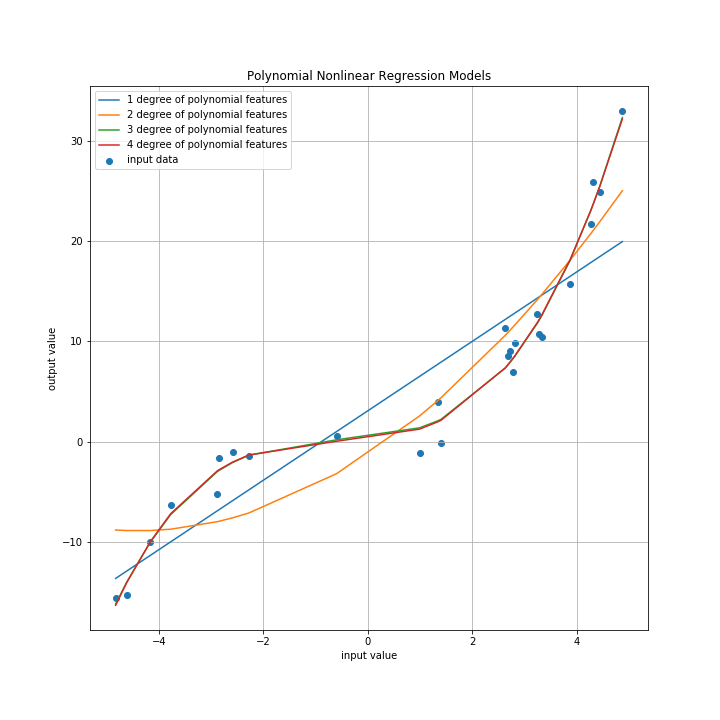
\includegraphics[width = 0.7\textwidth]{Question 2a.jpg}
\end{center}
\end{answerbox}



\end{subquestion}


%
%
\begin{subquestion}{(3 points) Create a bar plot where you display the Mean Squared Error of each of the four different polynomial regression models from the previous question.}


\begin{answerbox}{35em}
This image shows  Mean Squared Error of each of the four different polynomial regression models
\begin{center}
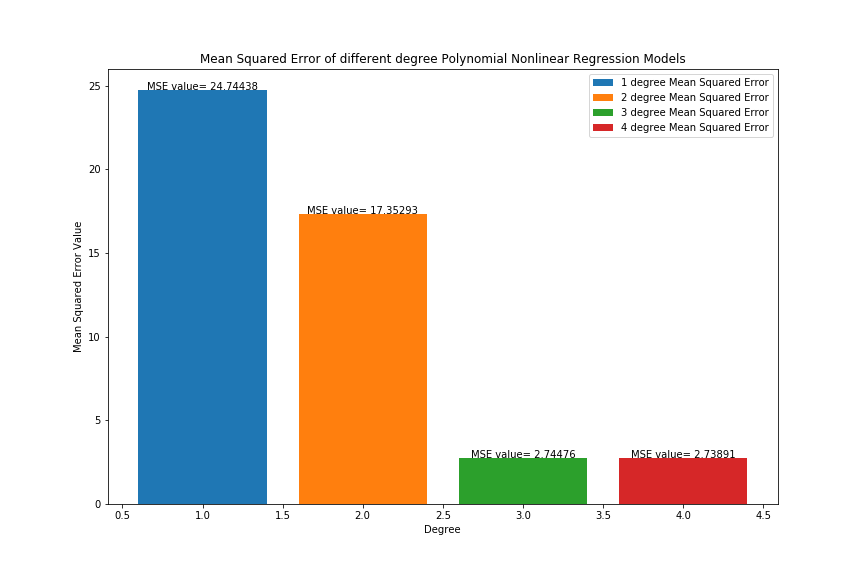
\includegraphics[width = 0.7\textwidth]{Question 2b.jpg}
\end{center}
\end{answerbox}



\end{subquestion}


%
%
\begin{subquestion}{(4 points) Comment on the fit and Mean Squared Error values of the $M=3$ and $M=4$ polynomial regression models. 
Do they result in the same or different performance? 
Based on these results, which model would you choose?}


\begin{answerbox}{15em}
I will choose M = 3. When M = 3, the MSE value is 2.7447567192524263 and when M = 4, the MSE value is 2.7389111790755374.
The advantage of choosing M = 4 is that the value of MSE is smaller than that of M = 3 which means M=4 has a better fitted model, better performace and higher accuracy. But the disadvantage of choosing M = 4 is that the value of MSE is not significantly lower and amount of computation is much higher,so the performance increase are not dramtically and consequently the computation increase. The advantage of choosing M = 3 is that it is a good fitted model and the amount of computation is reasonable. Hence, if the focus of the model on the accuracy and smaller MSE then choose M = 4, if the foucs is on appropriate accuracy and computation then choose M = 3.
\end{answerbox}


 
\end{subquestion}



%
%
\begin{subquestion}{(6 points) Instead of using polynomial basis functions, in this final part we will use another type of basis function - radial basis functions (RBF). 
Specifically, we will define $\boldsymbol{\phi}(x_i) = [1, rbf(x_i; c_1, \alpha), rbf(x_i; c_2, \alpha), rbf(x_i; c_3, \alpha), rbf(x_i; c_4, \alpha)]$, where $rbf(x; c, \alpha) =  \exp(-0.5(x-c)^2 / \alpha^2)$ is an RBF kernel with center $c$ and width $\alpha$. Note that in this example, we are using the same width $\alpha$ for each RBF, but different centers for each.\\ 
Let $c_1=-4.0$, $c_2=-2.0$, $c_3=2.0$, and $c_4=4.0$ and plot the resulting nonlinear predictions using the \texttt{regression\_part2.csv} dataset for $\alpha \in \{0.2, 100, 1000\}$. 
You can plot all three results on the same figure.
Comment on the impact of larger or smaller values of $\alpha$.
}


\begin{answerbox}{35em}
This image shows Radial Basis Function Model(RBF) in different alpha
\begin{center}
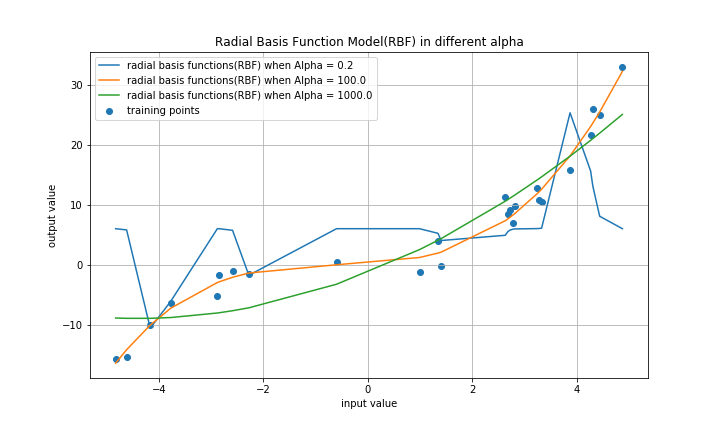
\includegraphics[width = 0.7\textwidth]{Question 2d.jpg}
\end{center}
When alpha = 100 is the best.Because this model is not overfit or underfit and MSE is the smallest one that means it is the most accurate one.
When alpha = 1000, the model become overfit and it's not accurate.This means that the noise or random fluctuations in the training data is picked up and learned as concepts by the model. The problem is that these concepts do not apply to new data and negatively impact the models ability to generalize.
When alpha = 0.2, the model is underfit.An underfit machine learning model is not a suitable model and will be obvious as it will have poor performance on the training data.
\end{answerbox}



\end{subquestion}



\end{question}






%%%%%%%%%%%%%%%%%%%%%%%%%%%%%%%%%%%%%%%%%%%%%%%%%%%%%%%%%%%%%%%%%%%%%%%%%%%%%%
%============================================================================%
%%%%%%%%%%%%%%%%%%%%%%%%%%%%%%%%%%%%%%%%%%%%%%%%%%%%%%%%%%%%%%%%%%%%%%%%%%%%%%
\clearpage


\begin{question}{(26 total points) Decision Trees}

\questiontext{In this question we will train a classifier to predict if a person is smiling or not.}




%
%
\begin{subquestion}{(4 points) Load the data, taking care to separate the target binary class label we want to predict, \texttt{smiling}, from the input attributes. 
Summarise the main properties of both the training and test splits. 
}


\begin{answerbox}{12em}
Data in train: 4800 entries,range index is from 0 to 4799. 4800 rows and 138 columns. dtypes: float64(136), int64(1).
<class 'pandas.core.frame.DataFrame'>
RangeIndex: 4800 entries, 0 to 4799.  Columns: 137 entries, x0 to smiling
There are 68 groups(x,y) in database. 0 represent no smile and 1 represent smile. 
Memory usage: 5.0 MB

Data in test:1200 entries,range index is from 0 to 1199. 1200 rows and 138 columns. dtypes: float64(136), int64(1)
<class 'pandas.core.frame.DataFrame'>
RangeIndex: 1200 entries, 0 to 1199
Columns: 137 entries, x0 to smiling
There are 68 groups(x,y) in database. 0 represent no smile and 1 represent smile.
memory usage: 1.3 MB



\end{answerbox}



\end{subquestion}


%
%
\begin{subquestion}{(4 points) Even though the input attributes are high dimensional, they actually consist of a set of 2D coordinates representing points on the faces of each person in the dataset. 
Create a scatter plot of the average location for each 2D coordinate. One for (i) smiling and (ii) one not smiling faces. 
For instance, in the case of smiling faces, you would average each of the rows where \texttt{smiling = 1}. 
You can plot both on the same figure, but use different colors for each of the two cases. 
Comment on any difference you notice between the two sets of points. \\
\hint{Your plot should contain two faces.}
}


\begin{answerbox}{35em}
This image shows faces_train_image
\begin{center}
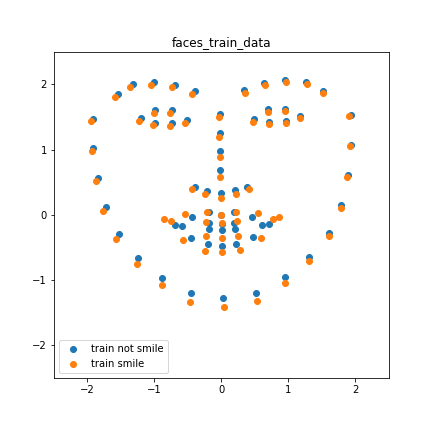
\includegraphics[width = 0.7\textwidth]{Question 3b.jpg}
\end{center}
The difference exist in the mouth edge. When the image is smiling then the edge is longer and more upward.





\end{answerbox}



\end{subquestion}


%
%
\begin{subquestion}{(2 points) 
There are different measures that can be used in decision trees when evaluating the quality of a split. 
What measure of purity at a node does the \href{https://scikit-learn.org/0.19/modules/generated/sklearn.tree.DecisionTreeClassifier.html}{DecisionTreeClassifier} in sklearn use for classification by default? 
What is the advantage, if any, of using this measure compared to entropy? 
}


\begin{answerbox}{10em}
In sklearn the decision tree use gini as default.Using gini is better than entropy because it doesn't need to calculate by log(). Hence it is also faster.
\end{answerbox}



\end{subquestion}


%
%
\begin{subquestion}{(3 points) 
One of the hyper-parameters of a decision tree classifier is the maximum depth of the tree. 
What impact does smaller or larger values of this parameter have? Give one potential problem for small values and two for large values. 
}


\begin{answerbox}{10em}
If the depth value is small, then it could be a shallow tree and a underfit model.In the shallow tree,we can say that the model has low variance since changing the sample does not change too much the model. It needs too many changed data points to be considered unstable. At the same time we can say that has a high bias, since it really can't represent the sine function which is the true model. We can say also that it has a low complexity.
If the depth is large, then it could be a over-complex tree and a overfit model.This model do not generalise the data well Consequently, practical decision-tree learning algorithms are based on heuristic algorithms such as the greedy algorithm where locally optimal decisions are made at each node. Such algorithms cannot guarantee to return the globally optimal decision tree. Also, when the depth is large,decision tree training is relatively expensive as the complexity and time taken are more.
\end{answerbox}



\end{subquestion}


%
%
\begin{subquestion}{(6 points) 
Train three different decision tree classifiers with a maximum depth of 2, 8, and 20 respectively.
Report the maximum depth, the training accuracy (in \%), and the test accuracy (in \%) for each of the three trees.
Comment on which model is best and why it is best. \\
\hint{Set \texttt{random\_state = 2001} and use the \texttt{predict()} method of the \href{https://scikit-learn.org/0.19/modules/generated/sklearn.tree.DecisionTreeClassifier.html}{DecisionTreeClassifier} so that you do not need to set a threshold on the output predictions.
You can set the maximum depth of the decision tree using the \texttt{max\_depth} hyper-parameter.}
}


\begin{answerbox}{20em}
In train database,when the depth is 2 the accuracy is 79.479\%. When the depth is 8 the accuracy is 93.354\%. When the depth is 20 the accuracy is 100\%.
In test database, when the depth is 2 the accuracy is 78.166\%. When the depth is 8 the accuracy is 84.083\%. When the depth is 20 the accuracy is 81.583\%.
When the depth is 8, the model is the best because the accuracy is the largest one, which means it's not overfit or underfit compared to others model. When the depth is 2,the accuracy is about 78\% which is slightly underfit and the accuracy is not large enough. When the depth is 20, the accuracy is about 81\% which is slightly decrease compared to the one which depth is 8. So when depth is 20, the model is overfit and decision tree training is relatively expensive as the complexity and time taken are more.
Hence the model which the depth is 8 is the best.
\end{answerbox}



\end{subquestion}


%
%
\begin{subquestion}{(5 points) 
Report the names of the top three most important attributes, in order of importance, according to the Gini importance from \href{https://scikit-learn.org/0.19/modules/generated/sklearn.tree.DecisionTreeClassifier.html}{DecisionTreeClassifier}. 
Does the one with the highest importance make sense in the context of this classification task? \\
\hint{Use the trained model with \texttt{max\_depth = 8} and again set  \texttt{random\_state = 2001}.}
}


\begin{answerbox}{10em}
The three most important attributes are x50,y48 and y29. It doesn't make sense even with highest importance because if the x50 deleted then x52 or others attributes with high imortance can replace x50 and become the highest importance. The 

\end{answerbox}



\end{subquestion}



%
%
\begin{subquestion}{(2 points) 
Are there any limitations of the current choice of input attributes used i.e. 2D point locations? If so, name one. 
}


\begin{answerbox}{10em}
Because it is a 2D image.The distance between the object and the camera is not obvious. Even if it is the same object,the input attribute will be different because of the distance. Also, the light and reflection light would also incerase the noise input when the distance is different.
\end{answerbox}



\end{subquestion}


\end{question}




%%%%%%%%%%%%%%%%%%%%%%%%%%%%%%%%%%%%%%%%%%%%%%%%%%%%%%%%%%%%%%%%%%%%%%%%%%%%%%
%============================================================================%
%%%%%%%%%%%%%%%%%%%%%%%%%%%%%%%%%%%%%%%%%%%%%%%%%%%%%%%%%%%%%%%%%%%%%%%%%%%%%%
\clearpage


\begin{question}{(14 total points) Evaluating Binary Classifiers}

\questiontext{In this question we will perform performance evaluation of binary classifiers.}




%
%
\begin{subquestion}{(4 points) Report the classification accuracy (in \%) for each of the four different models using the \texttt{gt} attribute as the ground truth class labels. 
Use a threshold of $>= 0.5$ to convert the continuous classifier outputs into binary predictions. 
Which model is the best according to this metric?
What, if any, are the limitations of the above method for computing accuracy and how would you improve it without changing the metric used?
}


\begin{answerbox}{15em}
alg_1 accuracy = 61.6\% 
alg_2 accuracy = 55.0\%
alg_3 accuracy = 32.1\%
alg_4 accuracy = 32.9\%
When I increase the threshold the accuracy will increase.
\end{answerbox}



\end{subquestion}



%
%
\begin{subquestion}{(4 points) Instead of using classification accuracy, report the Area Under the ROC Curve (AUC) for each model. 
Does the model with the best AUC also have the best accuracy? If not, why not?\\
\hint{You can use the  \href{https://scikit-learn.org/0.19/modules/generated/sklearn.metrics.roc\_auc\_score.html}{roc\_auc\_score} function from sklearn.}
}


\begin{answerbox}{15em}
Area Under the ROC Curve (AUC) in alg_1 = 0.732093
Area Under the ROC Curve (AUC) in alg_2 = 0.631628
Area Under the ROC Curve (AUC) in alg_3 = 0.063950
Area Under the ROC Curve (AUC) in alg_4 = 0.847387
The model alg_4 is the best. Because 



\end{answerbox}



\end{subquestion}



%
%
\begin{subquestion}{(6 points) Plot ROC curves for each of the four models on the same plot.
Comment on the ROC curve for \texttt{alg\_3}?
Is there anything that can be done to improve the performance of \texttt{alg\_3} without having to retrain the model?\\
\hint{You can use the \href{https://scikit-learn.org/0.19/modules/generated/sklearn.metrics.roc\_curve.html}{roc\_curve} function from sklearn.}
}


\begin{answerbox}{35em}





\end{answerbox}



\end{subquestion}

\end{question}







\end{document}